\chapter{RVM, India, and ...}
\label{chap6}

In the previous chapter, through regorous analysis we find RVM to be a powerful tool to predict the scaled margin distribution of elections. Furthermore, we demonstrated that voter turnouts play a fundamental role in driving the margins and, together with a proposed random voting model (RVM), can accurately predict the scaled distribution of victory margins. This robust connection between turnouts and margins holds across multiple elections and electoral scales. These findings naturally raise the question: Can the distribution of other relevant electoral statistics be uncovered using voter turnout distributions?

In this Letter, using empirical data from Indian elections \cite{india_data, lokdhaba} spanning several decades and vastly different electoral scales, we demonstrate a strong correlation between the distributions of votes received by winners and runner-ups and voter turnouts. Leveraging this correlation and the RVM, we analytically predict the scaled distributions of the votes secured by winners and runner-ups using the corresponding turnout distributions. This prediction remarkably holds good at all the electoral scales -- from large parliamentary constituencies ($ \sim 10^6$ voters) down to the smallest polling booth levels ($\sim 10^2-10^3$ voters). Further, we show a rather surprising scale invariance of the margin distributions, a characteristic typical of Indian elections. Finally, a robust universality in the distribution of scaled margin-to-turnout ratio is demonstrated, strengthening our recent proposition.

We formalize our framework as follows: An {\it election} happens at all the $N$ electoral units following the first-post-the-past principle \cite{johnston2007politics}. Let the $i$-th electoral unit have $n^c_i$ candidates and $n^v_i$ eligible voters, where $i=1,2, \dots N$. Usually, only a fraction of the eligible voters cast their votes. This is termed the turnout $T_i \le n^v_i$. It is a direct indicator of the people's interest in the electoral process, and its distribution $g(T)$ encodes information about electoral statistics \cite{pal2024universal}. Let $v_{i,1}, v_{i,2}, \dots, v_{i,n^c_i}$ be the votes secured by $n^c_i$ candidates such that $\sum_j v_{i,j}=T_i$. The candidate securing the highest number of votes, $V_{w}$, is declared the winner, while the candidate with the second-highest votes, $V_{r}$, is the runner-up. By definition $V_w > V_r$. Further, the \emph{margin} of victory is defined as $M_i = V_{i, w} - V_{i, r}$, and indicates the extent of electoral competition.
\begin{table}[b]
\caption{\label{tab:example}Electoral units in various elections in India}
\begin{ruledtabular}
\begin{tabular}{llll}
Type & Type of electoral unit & Type of election & Size \\
\hline
GE-PB & Polling booth & General election  &  $10^3$ \\
GE-AC & Assembly constituency & General election  &  $10^5$ \\
GE-PC & Parliamentary constituency & General election  &  $10^6$ \\
SE-AC & Assembly constituency & State election  &  $10^5$ \\
\end{tabular}
\end{ruledtabular}
\label{table1}
\end{table}

The electoral units in this work have three distinct scales in terms of the size of the electorate: (i) parliamentary constituency (PC, largest scale), (ii) assembly constituency (AC, intermediate scale), and (iii) polling booth (PB, smallest scale). Table \ref{table1} describes the granularity of election data used in this work -- electoral units and their typical electorate size. While for the national-level general elections, we employ data from 3 different electoral scales (PC, AC, and PB), we use AC-level data for state elections. Depending on the electoral level considered, the winner and runner-up vote distributions have vastly different scales, with the winner vote distribution having wider support than the runner-up. However, when both distributions are scaled by their respective mean values (mean taken over all elections for which data is available), the winner and runner-up vote distributions -- $Q_{\widetilde{V_w}}(\widetilde{V_w})$ and $Q_{\widetilde{V_r}}(\widetilde{V_r})$ -- explicitly display a strong correlation with the corresponding scaled turnout distributions $Q_{\widetilde{T}}(\widetilde{T})$. Note that any variable $Y$, scaled by their mean $\langle Y \rangle$, is denoted by $\widetilde{Y} = Y / \langle Y \rangle$. Figure \ref{fig:1} displays this key result at four electoral units described in Table \ref{table1}. Remarkably, at larger electoral scales (PC and AC), not only the tail but the entire scaled distributions of winner and runner-up votes mimic the corresponding scaled turnout distribution as seen in Fig. \ref{fig:1}(b-d). This strong correlation indicates that the turnout distribution contains crucial information about different election statistics and can be leveraged to predict the scaled vote distributions of the winner and the runner-up. To explore this possibility, we employ our recently proposed random voting model (RVM) \cite{pal2024universal}, which is demonstrably effective at predicting the scaled distribution of several election statistics, such as the \emph{margin} of victory.

\begin{figure}[t]
    \centering
    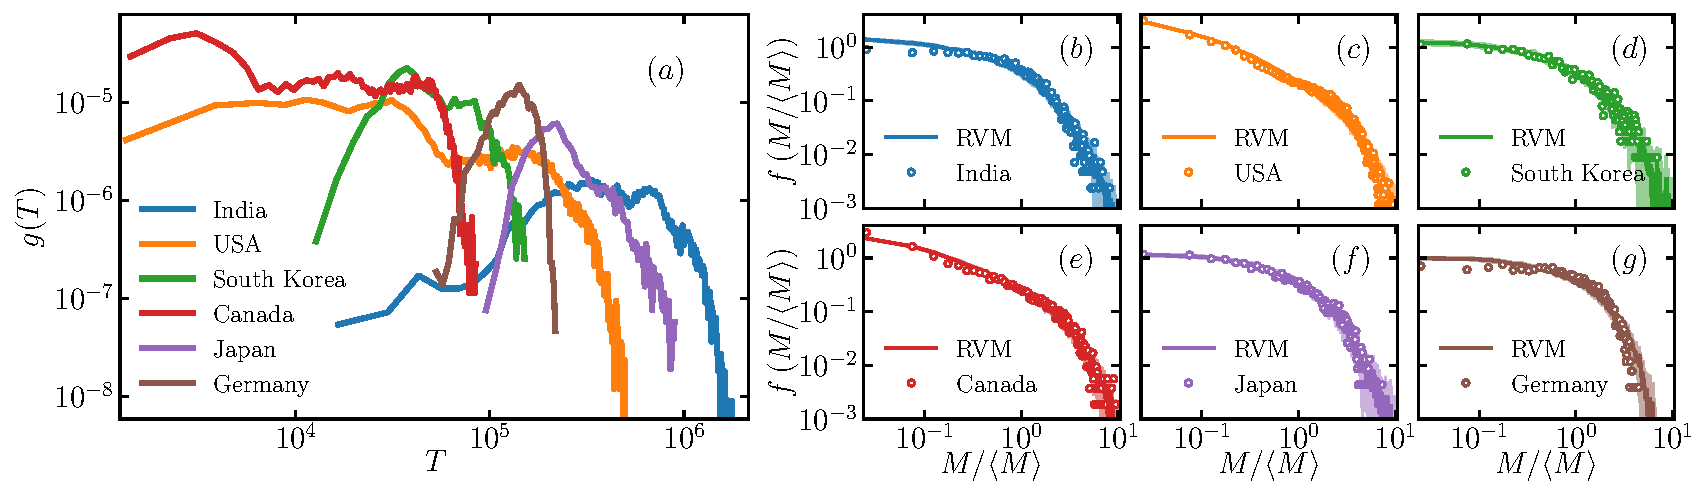
\includegraphics[width=\columnwidth]{fig_1.pdf}
    \caption{Winner, runner-up vote distributions, and turnout distributions, scaled by their respective means. Notably, at larger electoral scales (AC / PC), the winner and runner-up distributions mimic the corresponding turnout distribution.}
    \label{fig:1}
\end{figure}

\begin{figure*}[t]
    \centering
    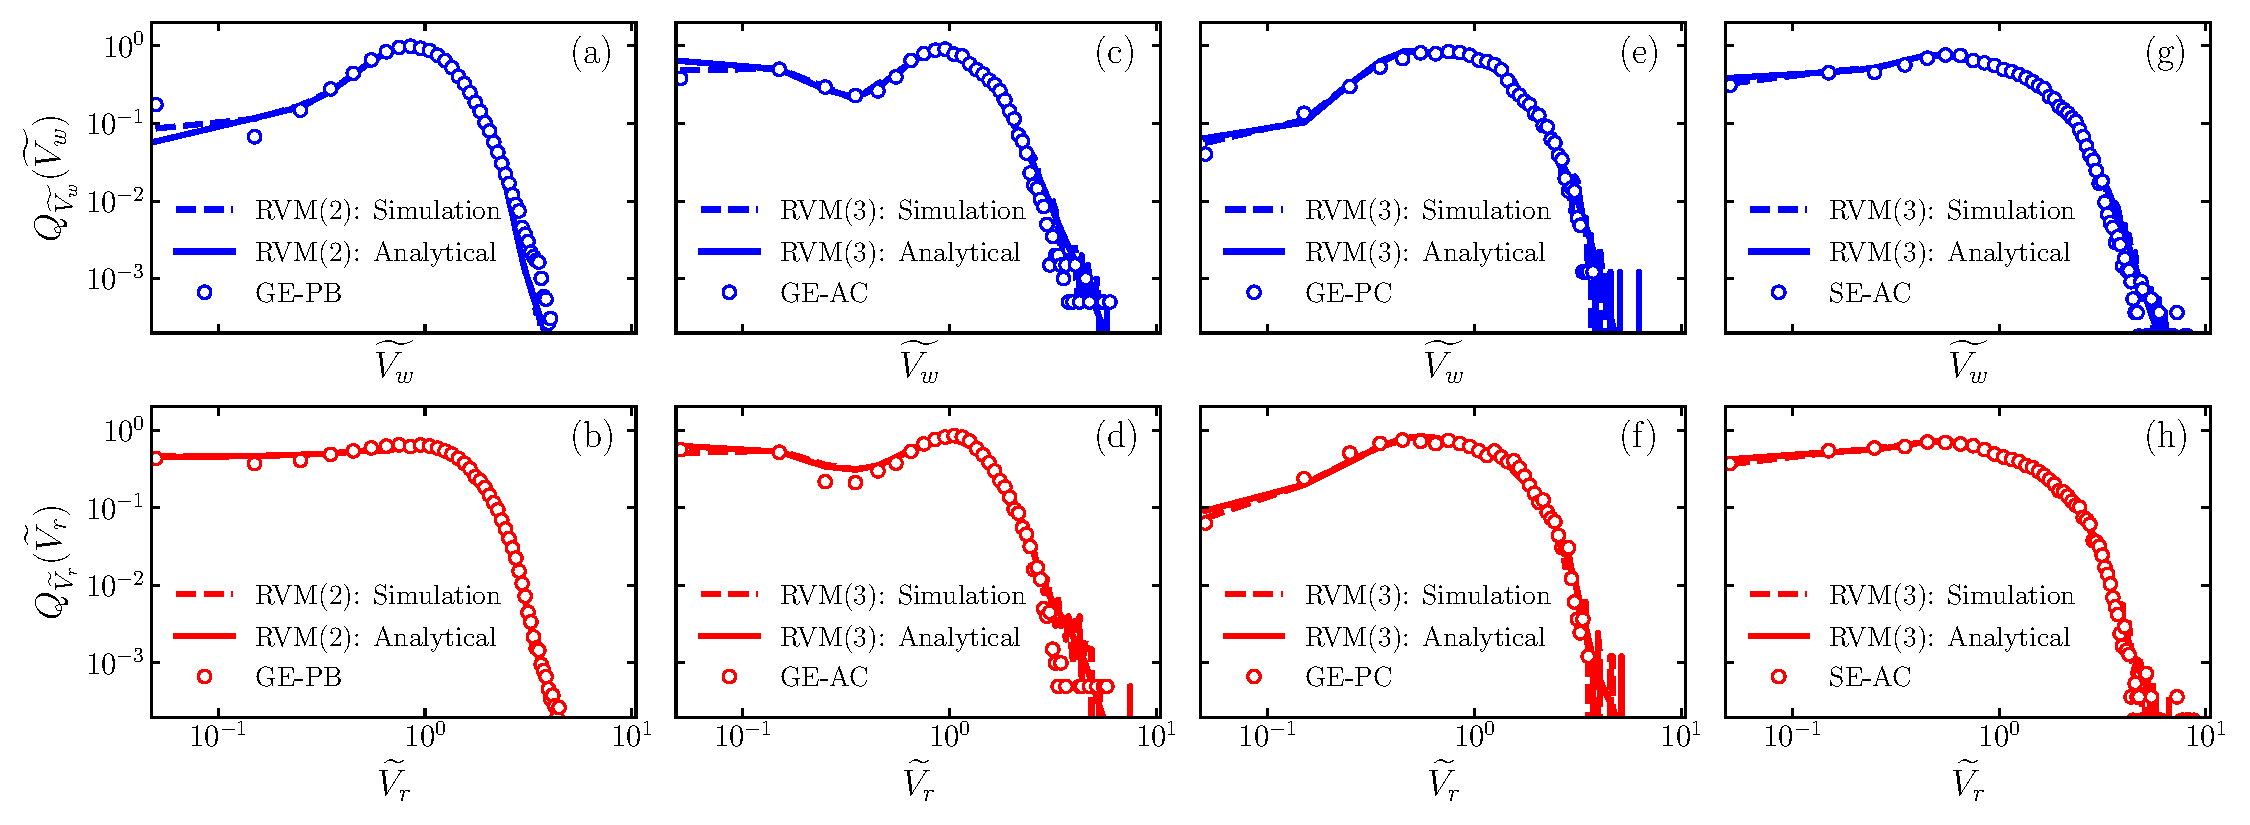
\includegraphics[width=\linewidth]{fig_2.pdf}
    \caption{Winner and runner-up vote distributions scaled by their respective means. Panels (a, b), (c, d), and (e, f) depict, respectively, the scaled winner and runner-up vote distribution at the polling booth, assembly constituency, and parliamentary constituency level for Indian general elections. Panels (g, h) correspond to the distributions for the state elections at the assembly constituency level. The analytical predictions (solid lines) are in remarkable agreement with the empirical distributions (open circle). Predictions from RVM simulations (dashed line) closely follow the analytical curves.}
    \label{fig:2}
\end{figure*}

The random voting model, later denoted as {RVM $(T, n^c)$}, is built around the framework of elections described above and consists of $N$ electoral units with $n^c_i$ number of candidates contesting for the votes of $T_i$ electors who have voted in the $i$-th electoral unit. Then, the probability that $j$-th candidate attracts electors' votes is:
\begin{equation}
    p_{ij} = \frac{w_{ij}}{\sum_{k=1}^{n^c_i} w_{ik}}, ~~~w_{ij} \sim \mathcal{U}(0, 1), ~~ (j = 1, 2, \cdots n^c_i).
    \label{eq:prob}
\end{equation}
In this, $\mathcal{U}(0, 1)$ is the uniform distribution. This model was shown to capture the various statistical features of empirical election data, such as the margin distributions and the universal features embedded in the election data \cite{pal2024universal}. In particular, the random voting model with $n^c = 3$ candidates -- {RVM $(T, 3)$} -- predicts the scaled distribution of \emph{margin} remarkably well, irrespective of electoral scales and countries \cite{pal2024universal}. In this work, we employ a refined approach based on the notion of the effective number of parties defined as \cite{laakso1979effective}:
\begin{equation}
    ^{(E)}n^c_i = \frac{1}{\sum_{k=1}^{n^c_i} (V_{ik} / T_{i})^2}.
    \label{eq:effc}
\end{equation}
In large elections exercise such as that in India, even though many candidates join the fray, a few corner most of the votes. For instance, if all the votes are garnered by just one candidate, then $V_{i1}=T_i$, and $V_{ij}=0$ for $j=2, \dots n^c$. In this case, $^{(E)}n^c_i=1$. However, if all the votes are split equally among two candidates, $^{(E)}n^c_i=2$, thus, Eq. \ref{eq:effc} captures the idea of an effective number of candidates in $i$-th electoral unit. Further, by averaging over all the electoral units, we obtain: 
\begin{equation}
    ^{(E)}\Tilde{n}^c =  \left[\frac{1}{N}\sum_{k=1}^{N}{}^{(E)}n^{c}_k \right],
\end{equation}
where $\left[\:*\:\right]$ denotes the operation of extracting the closest integer value. And $^{(E)}\Tilde{n}^c $ indicates the effective number of candidates for an entire election at different electoral scales. From empirical data of Indian elections at different scales, we find $^{(E)}\Tilde{n}^c = 2$ at the polling booth (PB-GE) level for the General Elections. However, for all the other three cases of AC-GE, PC-GE, and AC-SE, we obtain $^{(E)}\Tilde{n}^c = 3$. Now, we shall solve RVM $(T, n^c)$ for $n^c = 2$ and $n = 3$ to analytically describe the results observed in Fig. \ref{fig:1}.\\

The primary object of interest is the distribution of the votes received by the winner and the runner-up. In the large turnout limit, $T >> 1$, the votes received by $j$-th candidate can be approximated as $V_j \approx p_j T$ (index $i$ is dropped as we focus on a single electoral unit). Consequently, the vote share is defined as:
\begin{equation}
    v_j = V_j/T ~~ \text{with} ~ j = 1, 2, \dots n^c.
    \label{eq:voteshare}
\end{equation}

Thus, in this limit, the vote share distribution is effectively the same as the distribution of $p_j$. Recall that $p_j$ can be constructed from random weights using Eq.~\ref{eq:prob}. These weights are $n^c$ \emph{i.i.d.} random variables $\{w_1, w_2, \cdots, w_{n^c}\}$ drawn from the uniform distribution $\mathcal{U}(0, 1)$. When arranged in ascending order, the random variable at the $k$-th place is defined as the $k$-th order statistics and is denoted by $w^{n^c}_{(k)}$ \cite{BarBalNag2008}. Specifically, $w^{n^c}_{(1)}$ and $w^{n^c}_{(n^c)}$ represent the smallest and the largest weights, respectively. Then, the joint probability distribution function (jpdf) or all the order statistics is given by:
\begin{equation}
    \mathbbm{P}\left(w^{n^c}_{(1)}, w^{n^c}_{(2)}, ... w^{n^c}_{(n^c)}\right) = n^c!.
    \label{eq:jpdf1}
\end{equation}
Finally, the winner's vote share $v_w$ and runner-up's vote share $v_r$ can be expressed in terms of order statistics as:
\begin{equation}
    v_w = \frac{w^{n^c}_{(n^c)}}{\sum_{k = 1}^{n^c}w^{n^c}_{(k)}} ~~~\text{and}~~~ v_r = \frac{w^{n^c}_{(n^c - 1)}}{\sum_{k = 1}^{n^c}w^{n^c}_{(k)}}.
    \label{eq:voteshare_order_stat}
\end{equation}

Their distributions can be obtained from the jpdf in Eq.~\ref{eq:jpdf1} by integrating out the other variables (for detailed calculations, see Supplementary Material \cite{supp}). When the number of candidates $n^c = 2$, the distribution of the winner's vote share $P_{v_w}(v_w)$ is found to be:
\begin{equation}
{P_{v_w}(v_w) = }
\begin{dcases}
     \frac{1}{v_w^2}, ~~\text{ if } ~~ \frac{1}{2} < v_w < 1,\\
     0, ~~\text{ otherwise}.
\end{dcases}
\label{eq:wdist1}
\end{equation}
The vote share distribution of the runner-up can also be calculated similarly and is given by:
\begin{equation}
{P_{v_r}(v_r) = }
\begin{dcases}
     \frac{1}{(1- v_r)^2}, ~~\text{ if } ~~ 0 < v_r \leq \frac{1}{2},\\
     0, ~~\text{ otherwise}.
\end{dcases}
\label{eq:rdist1}
\end{equation}
The conditions in Eqs.~\ref{eq:wdist1}-\ref{eq:rdist1} reflect the intuitive idea that when there are only two candidates, the winner's vote share cannot be less than $1/2$, and the runner-up cannot exceed $1/2$. For $n^c = 3$, the winner's vote share distribution is:
\begin{equation}
P_{v_w}(v_w) = 
\begin{dcases}
     \frac{3v_w - 1}{ v_w^3}, ~~\text{ if } ~~\frac{1}{3} < v_w \leq \frac{1}{2}\\
     \frac{1 - v_w}{v_w^3}, ~~\text{ if } ~~\frac{1}{2} < v_w < 1\\
     0, ~~\text{ otherwise},
\end{dcases}
\end{equation}
and the distribution of the runner-up's vote share is:
\begin{equation}
{P_{v_r}(v_r) = }
\begin{dcases}
    \frac{v_r (2 - 3 v_r)}{(1 - v_r)^2 (1 - 2 v_r)^2}, ~~\text{ if } ~~ 0 < v_r \leq \frac{1}{3}\\
    \frac{1 - 2 v_r}{v_r^2(1 - v_r)^2}, ~~\text{ if } ~~ \frac{1}{3} < v_r \leq \frac{1}{2}\\
     0, ~~ \text{ otherwise}.
\end{dcases}
\end{equation}
The vote share distribution of the winner and the runner-up are defined as piecewise functions. They are non-zero when $\frac{1}{3} < v_w < 1$ and $0 < v_r \leq \frac{1}{2}$, respectively.
Based on Eq.~\ref{eq:voteshare}, the distribution of unscaled variables $Y = (V_w, V_r)$, given $T$, is related to the scaled variables $y = (v_w, v_r)$ via:
\begin{equation}
    \mathcal{P}(Y|T) = \frac{1}{T}P_y\left(\frac{Y}{T}\right),
    \label{eq:PYT}
\end{equation}
where $P_y(y)$ is the probability density function for the scaled variable, $y = (v_w, v_r)$. The distribution of $Y$ for arbitrary turnout distribution $g(T)$ is:
\begin{equation}
    Q_Y(Y) = \int g(T)~\mathcal{P}(Y|T)~dT, 
    \label{eq:QY}
\end{equation}
with $\langle Y \rangle = \int Y ~  Q_Y(Y)~dY$.
Finally, for the scaled variable $\widetilde{Y} = Y / \langle Y \rangle$, the distribution is:
\begin{equation}
    Q_{\widetilde{Y}}(\widetilde{Y}) =  \langle Y \rangle ~ Q_Y(\widetilde{Y}  \langle Y \rangle). 
    \label{eq:QYscaled}
\end{equation}
\begin{figure}[h!]
    \centering
    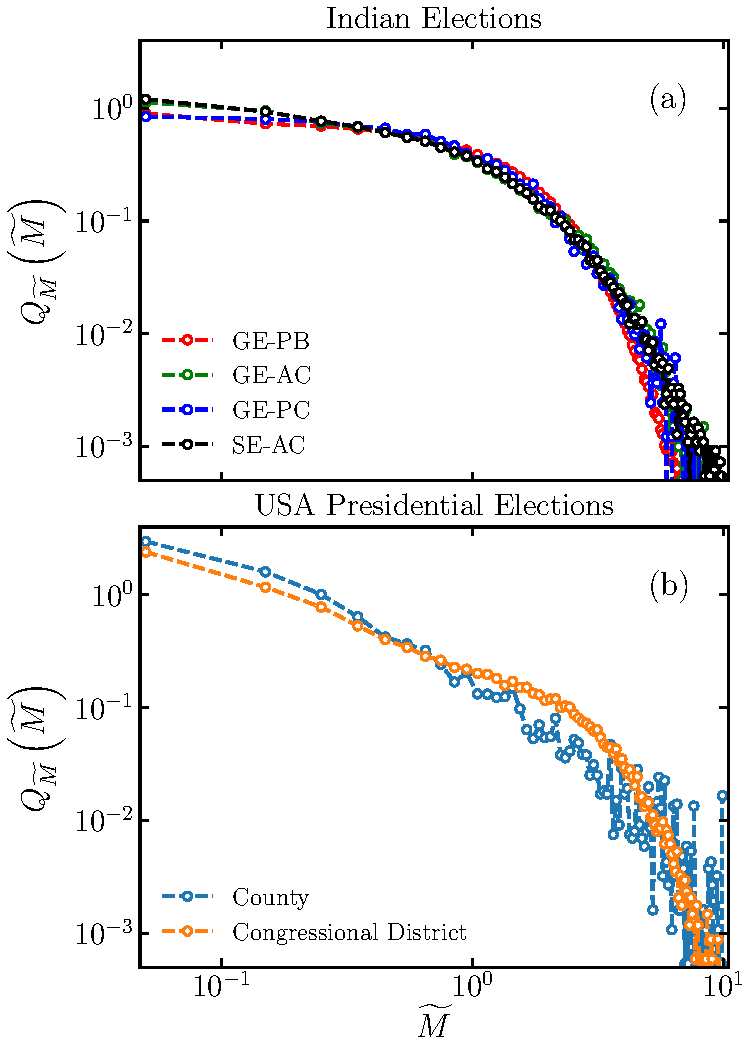
\includegraphics[width=1\linewidth]{fig_3.pdf}
    \caption{Margin distributions scaled by their respective means. (a) Data collapse in the scaled margin distributions of Indian elections at four electoral scales. (b) In contrast, such collapse is absent in the election data from the USA.}
    \label{fig:3}
\end{figure}
Using the empirical turnout distribution $g(T)$ from election data, Eq.~\ref{eq:QY} is numerically integrated. The resulting distribution is then scaled using Eq.~\ref{eq:QYscaled} to obtain the scaled distributions for the winner and runner-up vote shares, $ Q_{\widetilde{V_w}}(\widetilde{V_w})$ and $Q_{\widetilde{V_r}}(\widetilde{V_r})$, respectively. As demonstrated in Fig.~\ref{fig:2}, the analytical prediction (solid lines) is remarkably consistent with the empirical vote share distributions. The predictions from RVM simulations, which use the raw turnout data and $n^c = {^{(E)}\Tilde{n}^c}$ as inputs, closely follow the analytical distributions in Fig.~\ref{fig:2}. The scaled distributions of winner and runner-up votes depicted across all electoral scales, in Fig.~\ref{fig:2}, typically exhibit a power-law behavior in the tails for $\widetilde{V}_w, \widetilde{V}_r \gg 1$. Conversely, for $\widetilde{V}_w, \widetilde{V}_r \ll 1$, the distributions display different profiles. Remarkably, these differences are well captured by RVM predictions: RVM $(T, 2)$ accurately predicts distribution at the GE-PB level, while RVM $(T, 3)$ closely matches the distributions at the GE-AC, GE-PC, and SE-AC levels. Hence, the effective number of candidates (Eq.~\ref{eq:effc}) and the turnout distribution $g(T)$, when used within the RVM framework, successfully predict the winner and runner-up vote share distributions across distinct electoral scales.

Next, we consider the effect of voter turnouts $T$ on the \emph{margin} of victory $M$. To do this, firstly we define {\it specific margin} as $\mu = M / T = (V_w - V_r) / T$. In the large turnout $(T >> 1)$ limit, the specific margin can be expressed in terms of the order statistics of $w$ as:
\begin{equation}
    \mu = \frac{w^{n^c}_{(n^c)} - w^{n^c}_{(n^c - 1)}}{\sum_{k = 1}^{n^c}w^{n^c}_{(k)}},
\end{equation}
where $n^c$ is the number of candidates. Using the jpdf in Eq. \ref{eq:jpdf1}, for RVM $(T, 2)$ the distribution of specific margin can be obtained as (see Ref.~\cite{supp} for more details):
\begin{equation}
    P_{\mu}(\mu) = \frac{2}{(1 + \mu)^2},
\end{equation}
and for RVM $(T, 3)$, the distribution becomes:
\begin{equation}
    P_{\mu}(\mu) = \frac{(1 - \mu)(5 + 7\mu)}{(1 + \mu)^2(1 + 2\mu)^2}.
    \label{eq:24}
\end{equation}
Using Eq.~ \ref{eq:QY} - \ref{eq:QYscaled} and the empirical turnout distributions $g(T)$, the scaled margin distribution $Q_{\widetilde{M}}(\widetilde{M})$ can be obtained for the four different electoral scales which match the corresponding empirical distributions closely (see Ref.~\cite{supp}). Remarkably, the scaled distributions for the margin for Indian elections at four different scales collapse onto a single curve, as shown in Fig.~\ref{fig:3}(a). This data collapse is a direct consequence of the similarity in tail behavior in the corresponding turnout distributions (see Fig. \ref{fig:1}). This appears to be a characteristic of Indian elections and is not observed in most other countries. For instance, this data collapse is absent in the US elections for the empirical data at the County and Congressional district levels, as demonstrated in Fig.~\ref{fig:3} (b).
\begin{figure}[t]
    \centering
    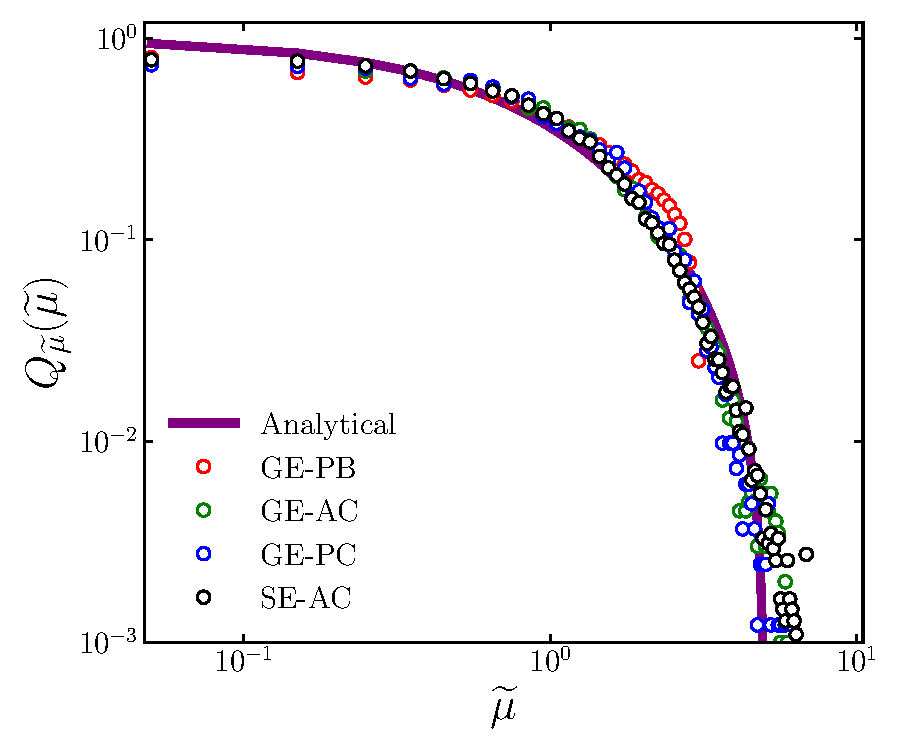
\includegraphics[width=1\linewidth]{fig_4.pdf}
    \caption{Specific margin distributions scaled by their respective means at distinct electoral scales in different types of Indian elections. The scaled specific margin distributions collapse on the analytical universal curve.}
    \label{fig:4}
\end{figure}

Recently, we have shown that the scaled distribution of specific margins $Q_{\widetilde{\mu}}(\widetilde{\mu})$, is universal irrespective of electoral scales and countries \cite{pal2024universal}. This universal distribution can be analytically obtained by rescaling Eq.~\ref{eq:24} with $\langle \mu \rangle = {1} / {2}+\ln \left({9 \sqrt[4]{3}} / {16}\right)$ (see Ref.~\cite{supp}). The empirical distributions from large election datasets are proposed to exhibit a better collapse to the analytical curve, as finite-size effects are suppressed. The presence of such universality helps us distill the complexity of the electoral processes in terms of universal behavior. As the electorate size in India is large (960 million in 2024) and datasets are available at various electoral scales, Indian elections provide the best test-bed to demonstrate such universality. Fig.~\ref{fig:4} demonstrates such universality. The distributions $Q_{\widetilde{\mu}}(\widetilde{\mu})$ at four distinct electoral scales (colored open circles) remarkably collapse onto the analytically predicted universal curve (solid line). This excellent collapse strengthens the proposition that in fairly conducted elections, the apparent deviation from universality can originate from finite data size.

In summary, elections are a source of excellent datasets for exploring collective decision-making by millions of people (interacting agents) at {\it distinct electoral scales}. However, most of the earlier works on elections have ignored the effects arising from differences in electoral scales. The voter turnout distribution $g(T)$ is a good indicator of the public trust and interest in the electoral process. Remarkably, we show that they also encode information about several crucial election statistics. Aided by election data from India -- the largest democracy in the world -- we demonstrate our results for different types of elections at multiple {\it distinct electoral scales}. Given the empirical $g(T)$ and an effective number of candidates for each electoral scale, we analytically obtain the scaled distributions of the winner and the runner-up votes using the framework of our recently proposed random voting model. The analytical predictions and the simulations are in excellent agreement with the empirical election data. Further, we demonstrate that the random voting model is effective in predicting the scaled margin distributions of Indian elections at vastly different electoral scales. Surprisingly, the scaled margin distribution remains invariant with respect to changes in electoral scales, making it a characteristic feature of Indian elections. Finally, the scaled specific margin distributions of Indian elections show a remarkable data collapse, strengthening the recently proposed universality \cite{pal2024universal}. This work paves the way for a wider understanding of electoral statistics from turnout distributions.
